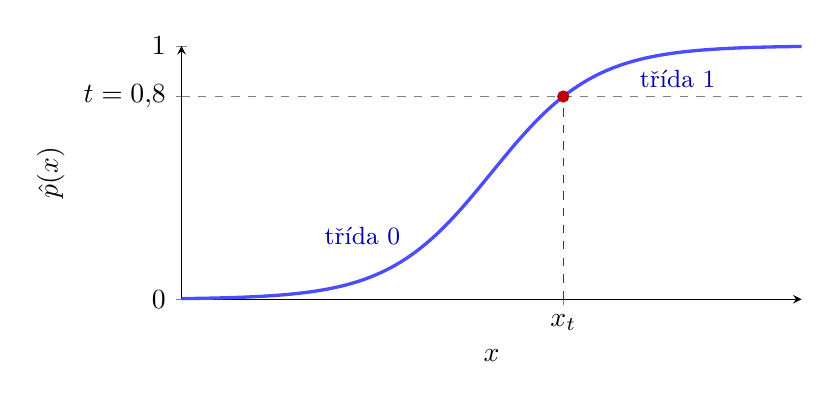
\begin{tikzpicture}
    \begin{axis}[
        width=0.78\textwidth,
        height=4.8cm,
        xmin=-6, xmax=6,
        ymin=0, ymax=1,
        axis lines=left,
        xlabel={$x$},
        ylabel={$\hat p(x)$},
        xtick={1.386},
        xticklabels={$x_t$},
        ytick={0,0.8,1},
        yticklabels={$0$,$t=0{,}8$,$1$},
        clip=false
    ]

        % Ukázka pro a=1, b=0 a t=0,8,
        % kdy x_t = ln(0,8/0,2) = ln 4.
        \addplot[
            very thick,
            blue!70,
            domain=-6:6,
            samples=120
        ] {1/(1+exp(-x))};

        \addplot[
            dashed,
            gray,
            domain=-6:6,
            samples=2
        ] {0.8};

        \addplot[
            dashed,
            red!75!black
        ] coordinates {
            (1.386,0)
            (1.386,0.8)
        };

        \addplot[
            only marks,
            mark=*,
            mark size=2pt,
            red!75!black
        ] coordinates {
            (1.386,0.8)
        };

        \node[
            font=\small,
            blue!70!black
        ] at (axis cs:-2.5,0.25) {třída~\(0\)};

        \node[
            font=\small,
            blue!70!black
        ] at (axis cs:3.6,0.87) {třída~\(1\)};

    \end{axis}
\end{tikzpicture}
